\theoremstyle{definition}
\newtheorem{theorem}{Beispiel}[section]

\chapter{Sequenzen}
\label{chp:sequences}
Bei den in dieser Arbeit verwendeten Datenstrukturen handelt es sich um \textit{Sequenzen}. Im Folgenden werden Sequenzen formal definiert und Begriffe zum Beschreiben dieser eingeführt. Daneben wird die binäre Sequenz als spezielle Abstraktion vorgestellt. Anschließend wird auf die zeitliche Korrelation zwischen Sequenzen eingegangen sowie Muster für eine Klassifizierung von Teilsequenzen definiert.

Zuerst wird allerdings noch ein Blick auf bestehende Definitionen für \textit{Sequenz} geworfen. Das Wort stammt aus dem Lateinischen und bedeutet Folge\footnote{ \cite{SequenzDuden}}. Allgemein versteht man darunter eine Folge von gleichartigen oder ähnlichen Dingen\footnote{ \cite{SequenzWiktionary}}. Der Duden definiert im Kontext der Computerwissenschaften zudem eine Sequenz als Folge von hintereinander gespeicherten Daten\footnote{ \cite{SequenzDuden}}. Da es sich bei Produktionsdaten um eben dies handelt, lässt sich der Begriff \textit{Sequenz} in dieser Arbeit verwenden. 

Bei den hier verwendeten Sequenzen handelt es sich um nominalskalierte Daten\footnote{ \cite{Stevens1946}}. Diese können weder in eine natürliche Reihenfolge gebracht werden, noch lassen sich Rechenoperationen wie Addition oder Multiplikation auf ihnen anwenden. Dies muss bei der weiteren Arbeit mit Sequenzen bedacht werden.

\section{Stand der Forschung}
\label{chp:state-of-research-sequences}
Den aktuellen Stand der Forschung und bisher geleistete Arbeit in diesem Gebiet sind nicht einfach herauszuarbeiten. Besonders im Bereich der Wissensgenerierung aus Produktionsdaten gestaltet es sich schwer Grundlagenliteratur zu finden. Ein Großteil der Veröffentlichungen beschäftigt sich auf einem höheren Level mit diesem Thema. Dagegen gibt es mehr wissenschaftliche Grundlagenliteratur im Bereich der Bioinformatik, die sich mit diesem Thema auseinandersetzt. Unter dem Stichwort \textit{Sequenzanalyse} findet man bspw. Algorithmen zur Analyse von DNA/RNA oder grundlegende Definitionen zum Umgang mit Sequenzen\footnote{ Siehe: \cite{Algoseq2014}}.

Die Ergebnisse der Literaturrecherche befindet sich im Anhang \ref{attachement:literature-research}. 

\section{Allgemeine Definitionen}
\label{chp:definitions-sequences}
Zur Simulation von Realdaten werden Sequenzen als eine endliche Menge von zeitdiskreten Ereignissen beschrieben. Ein Ereignis wird durch ein \textit{Symbol} repräsentiert. Die Zusammenfassung aller  Symbole einer Sequenz nennt man \textit{Alphabet} und wird durch $\Sigma$ dargestellt.

\begin{theorem}
Alphabet mit den Symbolen 0, 1 und 2: $\Sigma_1 = [0,1,2]$ oder mit den Symbolen a und b: $\Sigma_2 = [a,b]$. 
\end{theorem}

Eine Sequenz besitzt zudem eine Indexmenge $I$. Diese ist eine endliche linear geordnete Menge von 0 bis $n-1$ mit der Mächtigkeit $n$. Diese entspricht der Länge der Sequenz.

\begin{theorem}
Indexmenge $I = [0,1,2,...,n-1]$ mit der Mächtigkeit $|I| = n$.
\end{theorem}

Somit lässt sich eine Sequenz als Funktion $s : I \rightarrow \Sigma$ schreiben. Jedem Element der Menge $I$ (Index) wird ein Symbol des Alphabets $\Sigma$ zugeordnet.

\begin{theorem}
Aus $\Sigma = [a,b]$ und $n = 5$ folgt $s = [a,b,a,a,b]$.
\end{theorem}

Einen zusammenhängenden Bereich einer Sequenz bezeichnet man mit \textit{Teilsequenz} $t_{i,j}(s) = s[i,...,j]$. Mit Hilfe von Teilsequenzen lassen sich Sequenzen detaillierter betrachten. Bei zeitdiskreten Datenströmen lassen sich so bestimmte Zeiträume ohne den Einfluss vorheriger oder folgender Ereignisse betrachten. 

\begin{theorem}
Aus $s = [0,0,0,0,1,0,1,0,1]$ folgt $t_{4,8}(s) = [1,0,1,0,1] $.
\end{theorem}

Weiterhin lassen sich Sequenzen anhand ihrer Dimensionen beschreiben. Während eindimensionale Sequenzen an einer Stelle im Index nur einen Wert haben, haben mehrdimensionale Sequenzen mehr als einen Wert. In der Realität würde dies bspw. bedeuten, dass zu einem Zeitpunkt mehrere Informationen zum Zustand einer Maschine erfasst werden. Deshalb bietet es sich an, für jede Dimension ein eigenes Alphabet aufzustellen.

\begin{theorem}
Eine Sequenz mit den Alphabeten $\Sigma_{1} = [a,b]$ für die erste und $\Sigma_{2} = [A,B,C]$ für die zweite Dimension: $s = [\{a,C\},\{b,B\},\{a,B\},\{a,A\}]$.
\end{theorem}

\section{Binäre Sequenzen}
\label{chp:binary-sequences}
Auf Grundlage der formalen Beschreibung wird für die folgende Arbeit die binäre Sequenz eingeführt. Eine binäre Sequenz ist eindimensional und kann zwei mögliche Zustände besitzen. Dazu wird das Alphabet $\Sigma = [0,1]$ mit 0 für \textit{keinen Fehlerzustand} und 1 für \textit{Fehlerzustand} eingeführt.

Ziel dieses Ansatzes ist eine größtmögliche Vereinfachung von Realdaten zu erzielen. Es wird angenommen, dass der Betrieb einer Produktionsmaschine sich entweder in einem gewünschten oder unerwünschten Zustand befindet. Unter letzterem versteht man jegliches ungeplante Verhalten, weshalb Vorgänge, wie bspw. das Umrüsten einer Maschine als erwünschten und somit fehlerfreien Zustand gezählt werden. 

\begin{figure}[H]
	\centering
	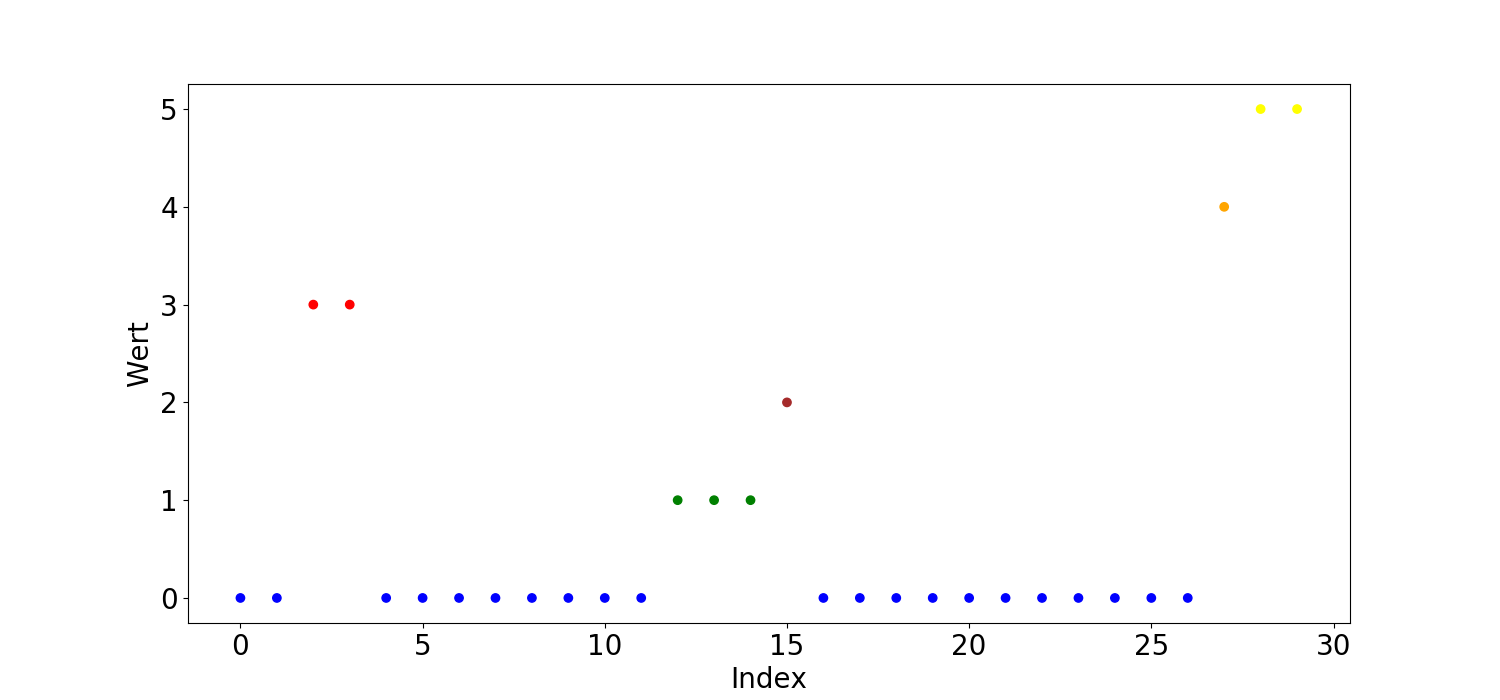
\includegraphics[scale=0.32]{images/sequences/binary-sequences-full}
	\caption{Sequenz mit sechs Zuständen}
	\label{fig:binary-sequences-full}
\end{figure}

In Abbildung \ref{fig:binary-sequences-full} sieht man eine Sequenz mit sechs möglichen Zuständen. Die Werte 0, 1, 2 stehen dabei für ein fehlerfreies und die Werte 3, 4, 5 für ein fehlerhaftes Verhalten der Produktionsmaschine. Durch das Zusammenfassen in diese beiden Kategorien, wird eine Vereinfachung der Sequenz erziehlt (vgl. Abbildung \ref{fig:binary-sequences-reduced}). Das die Reduktion auf zwei Zustände mit einem gewissen Informationsverlust einhergeht, muss bei der weiteren Arbeit mit den Sequenzen beachtet werden.

\begin{figure}[H]
	\centering
		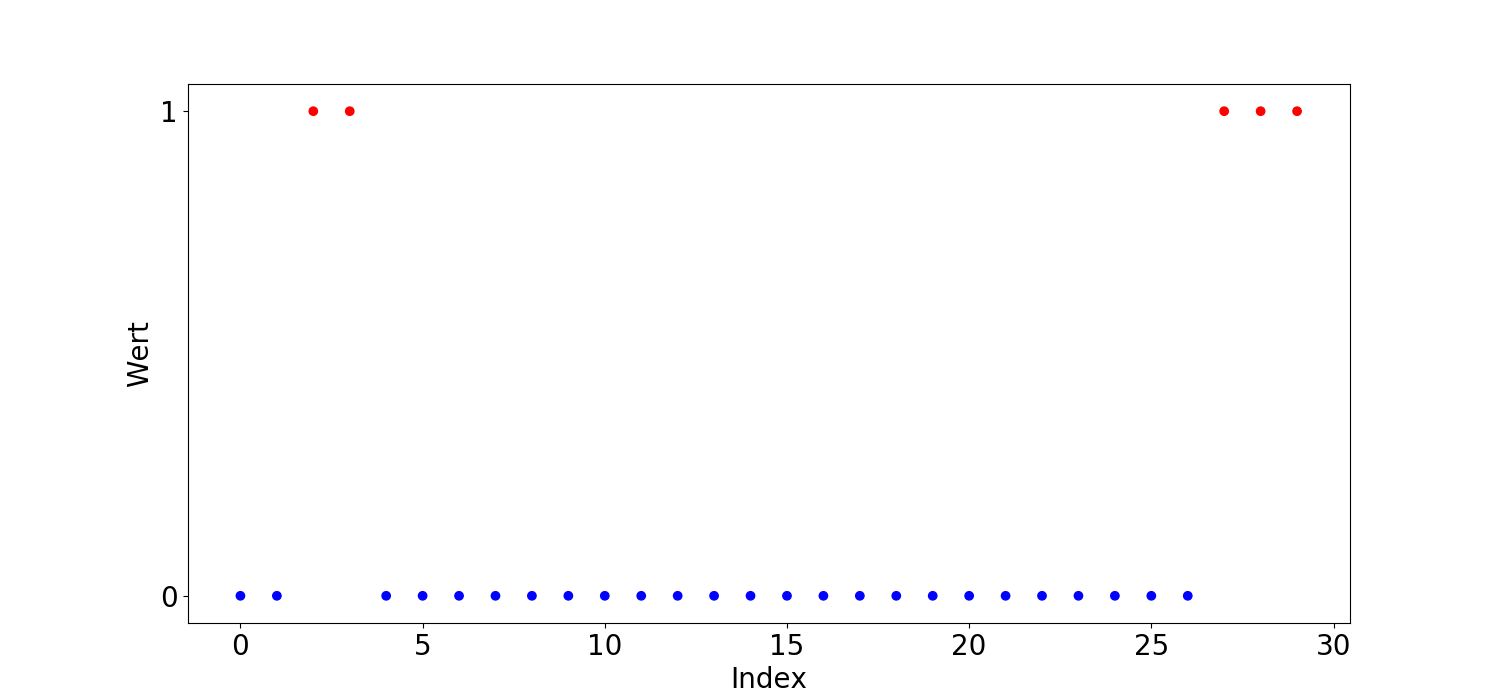
\includegraphics[scale=0.32]{images/sequences/binary-sequences-reduced}
	\caption{Sequenz mit zwei Zuständen}
	\label{fig:binary-sequences-reduced}
\end{figure}

\section{Eigenschaften}
\label{chp:properties-sequences}
Um Sequenzen oder Teilsequenzen zu klassifizieren, müssen Eigenschaften definiert und voneinander abgegrenzt werden. Dazu werden die \textit{Balance} und \textit{Frequenz} einer Sequenz eingeführt.

\subsubsection{Balance}

Mit der Balance wird das Verhältnis des Vorkommens eines Symbols zur Länge der Sequenz beschrieben. 

\begin{equation}
\label{eq:properties-sequences-balance}
Balance(Symbol) = \frac{Anzahl(Symbol)}{Gesamtl\ddot{a}nge\ der\ Sequenz}
\end{equation}

\begin{equation}
\label{eq:properties-sequences-binary-balance}
Balance(0) + Balance(1) = 1;\ f\ddot{u}r\ \Sigma = [0,1]
\end{equation}

Man kann die Balance somit auch als Maß für die Ausrichtung einer Sequenz zu einem Symbol hin bezeichnen. Die Balance wird nach der Formel \ref{eq:properties-sequences-balance} berechnet. Für eine binäre Sequenz gilt zudem Formel \ref{eq:properties-sequences-binary-balance}. Mit ihr ist es möglich Balance(1) aus Balance(0) und anders herum zu berechnen.

\begin{theorem}
Gegeben sind:
\begin{itemize}[noitemsep]
	\item Sequenz: $s = [1,0,0,0,1,0,1,1,1,1]$
	\item Alphabet: $\Sigma = [0,1]$
	\item Länge: $|s| = 10$
\end{itemize}
Daraus folgt:
\begin{itemize}
	\item [] $Balance(0) = \frac{Anzahl(0)}{|s|} = \frac{4}{10} = 0.4$
	\item [] $Balance(1) = 1 - Balance(0) = 1 - 0.4 = 0.6$
\end{itemize}
\end{theorem}

\subsubsection{Frequenz}

Daneben ist die Frequenz ein Maß für die Aktivität an Wertewechseln innerhalb einer Sequenz. Sie ist das Verhältnis zwischen der Anzahl an Wertewechsel und der Sequenzlänge. Sie wird nach Formel \ref{eq:properties-sequences-frequency} berechnet. 

\begin{equation}
\label{eq:properties-sequences-frequency}
Frequenz = \frac{Anzahl\ der\ Wertewechsel}{Gesamtl\ddot{a}nge\ der\ Sequenz}
\end{equation}

Ein Wertewechsel tritt auf, wenn ein Element der Sequenz sich von seinem Nachfolger unterscheidet, also $s_{i} \neq s_{i+1}$ ist. In einem Produktionsprozess könnte dies der Zeitpunkt sein, bei dem es zu einer Störung kommt, bzw. diese behoben wurde. Bei einer binären Sequenz handelt es sich um den Wechsel von 0 auf 1 oder von 1 auf 0.

\begin{theorem}
Gegeben sind:
\begin{itemize}[noitemsep]
	\item Sequenz: $s = [1,0,0,0,0,0,1,1,1,1]$
	\item Alphabet: $\Sigma = [0,1]$
	\item Länge: $|s| = 10$
\end{itemize}
Daraus folgt:
\begin{itemize}[noitemsep]
	\item [] $Frequenz = \frac{Anzahl\ der\ Wertewechsel}{|s|} = \frac{2}{10} = 0.2$
\end{itemize}
\end{theorem}

Somit lassen sich mit Hilfe der Balance und Frequenz Aussagen darüber treffen, wie oft ein Fehlerzustand in einer Sequenz auftritt und ob es häufig zu Wertewechseln kommt. 

\subsubsection{Teilsequenzen}

Dabei bietet es sich an, besonders bei langen Sequenzen, sich auch die Eigenschaften von Teilsequenzen anzuschauen. Das folgende - etwas größere - Beispiel soll dies verdeutlichen.

\begin{theorem}
Gegeben sind:
\begin{itemize}[noitemsep]
	\item Sequenz: $s = [0,0,0,0,0,0,0,0,1,1,1,1,1,1,1,1,1,1,1,1,0,1,0,1,0,1,0,1,0,1]$
	\item Alphabet: $\Sigma = [0,1]$
	\item Länge: $|s| = 30$
	\item Teilsequenzen: $t_{0,5}(s)$, $t_{6,11}(s)$, $t_{12,17}(s)$, $t_{18,23}(s)$ und $t_{24,29}(s)$
\end{itemize}
Daraus folgt mit den Formeln \ref{eq:properties-sequences-balance} und \ref{eq:properties-sequences-frequency} für jede Teilsequenz sowie die gesamte Sequenz:

\begin{center}
	\begin{tabular}{|c c c|}
		\hline
		Sequenz & Balance(0) & Frequenz \\
		\hline\hline
		s & $0.4\overline{3}$ & $0.3\overline{6}$ \\ 
		\hline
		$t_{0,5}(s)$ & 1 & 0 \\ 
		\hline
		$t_{6,11}(s)$ & $0.\overline{3}$ & $0.1\overline{6}$ \\
		\hline
		$t_{12,17}(s)$ & 0 & 0 \\
		\hline
		$t_{18,23}(s)$ & $0.\overline{3}$ & $0.\overline{6}$ \\
		\hline
		$t_{24,29}(s)$ & 0.5 & $0.8\overline{3}$ \\
		\hline
	\end{tabular}
\end{center}

Es zeigt sich, dass Balance und Frequenz in den Teilsequenzen teils stark variieren. Damit ergibt sich auch die Wichtigkeit, Sequenzen nicht nur als Ganzes, sondern auch deren Verhalten über die Zeit zu betrachten. So treten bis Index 12 immer mehr Fehlerzustände auf und werden ab Index 17 wieder weniger (vgl. Abbildung \ref{fig:properties-subsequences-balance}). Bei der Frequenz zeigen sich zu Beginn noch keine Wertewechsel, während zum Ende hin die Sequenz sehr aktiv wird (vgl. Abbildung \ref{fig:properties-subsequences-frequency}).

\begin{figure}[H]
	\centering
	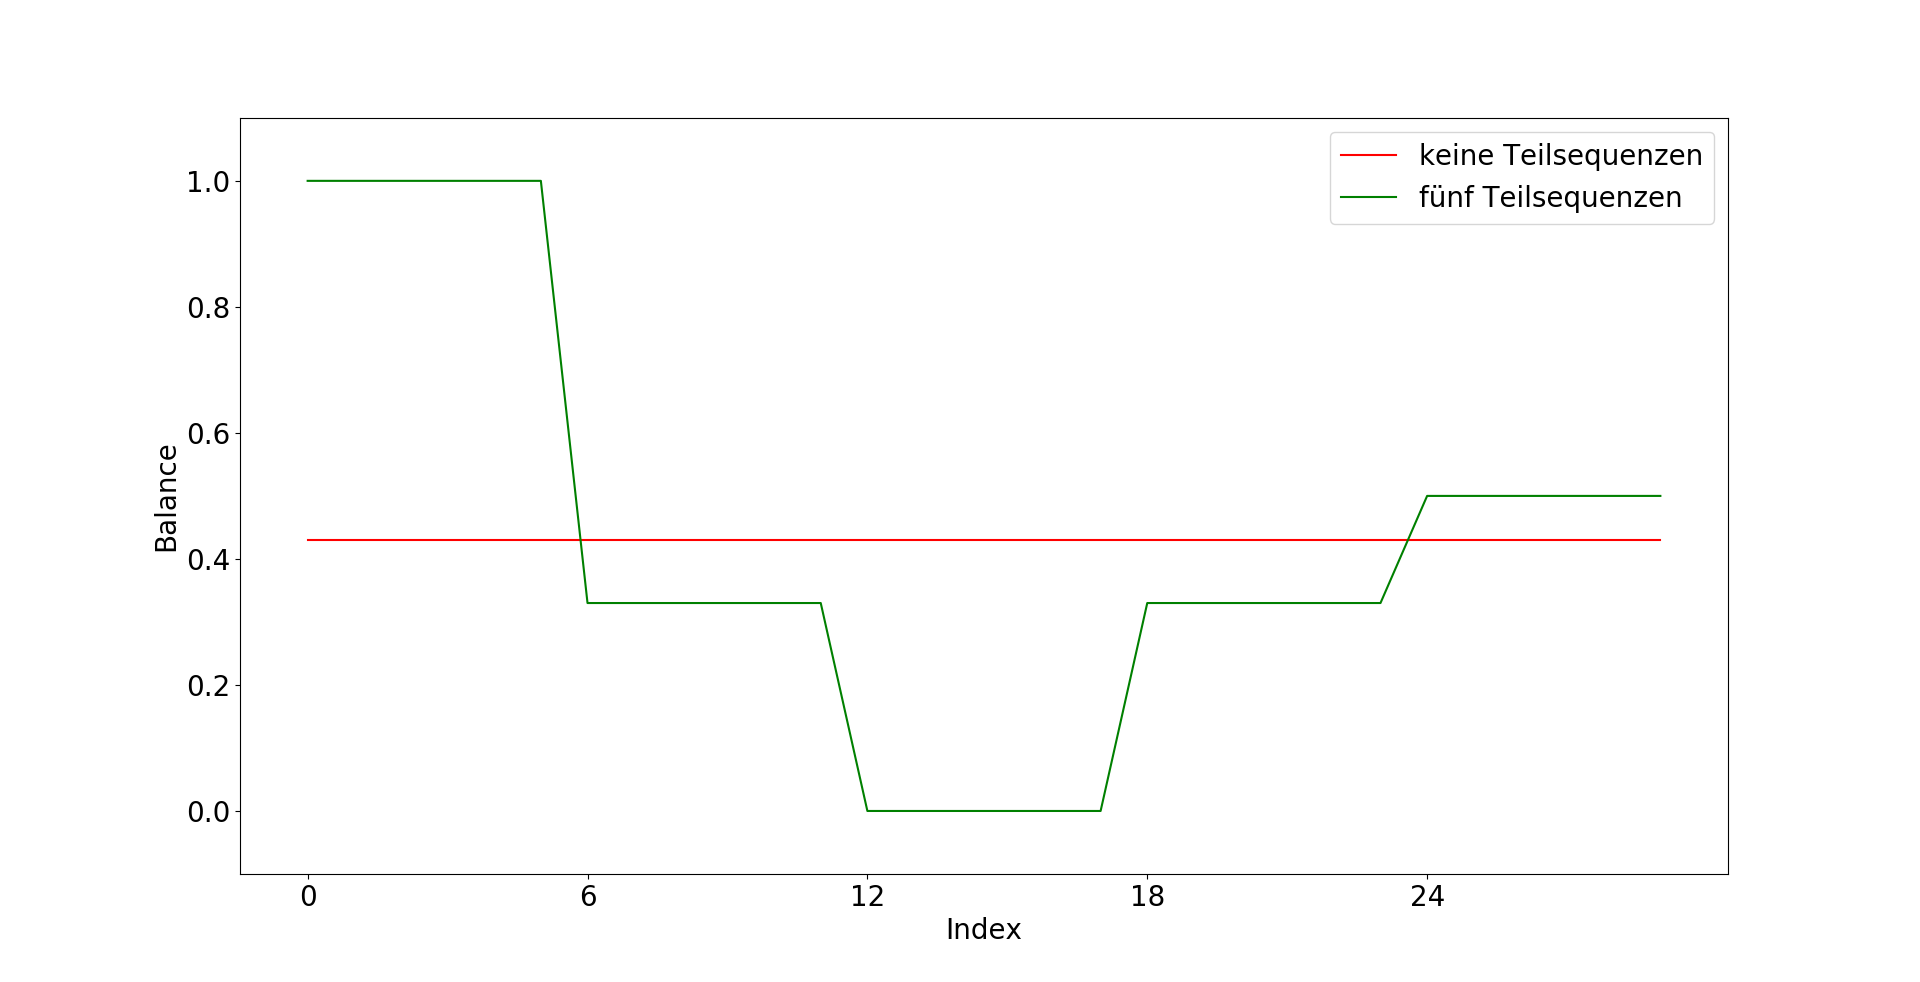
\includegraphics[scale=0.32]{images/sequences/subsequences-balance}
	\caption{Balance ohne und mit fünf Teilsequenzen}
	\label{fig:properties-subsequences-balance}
\end{figure}

\begin{figure}[H]
	\centering
	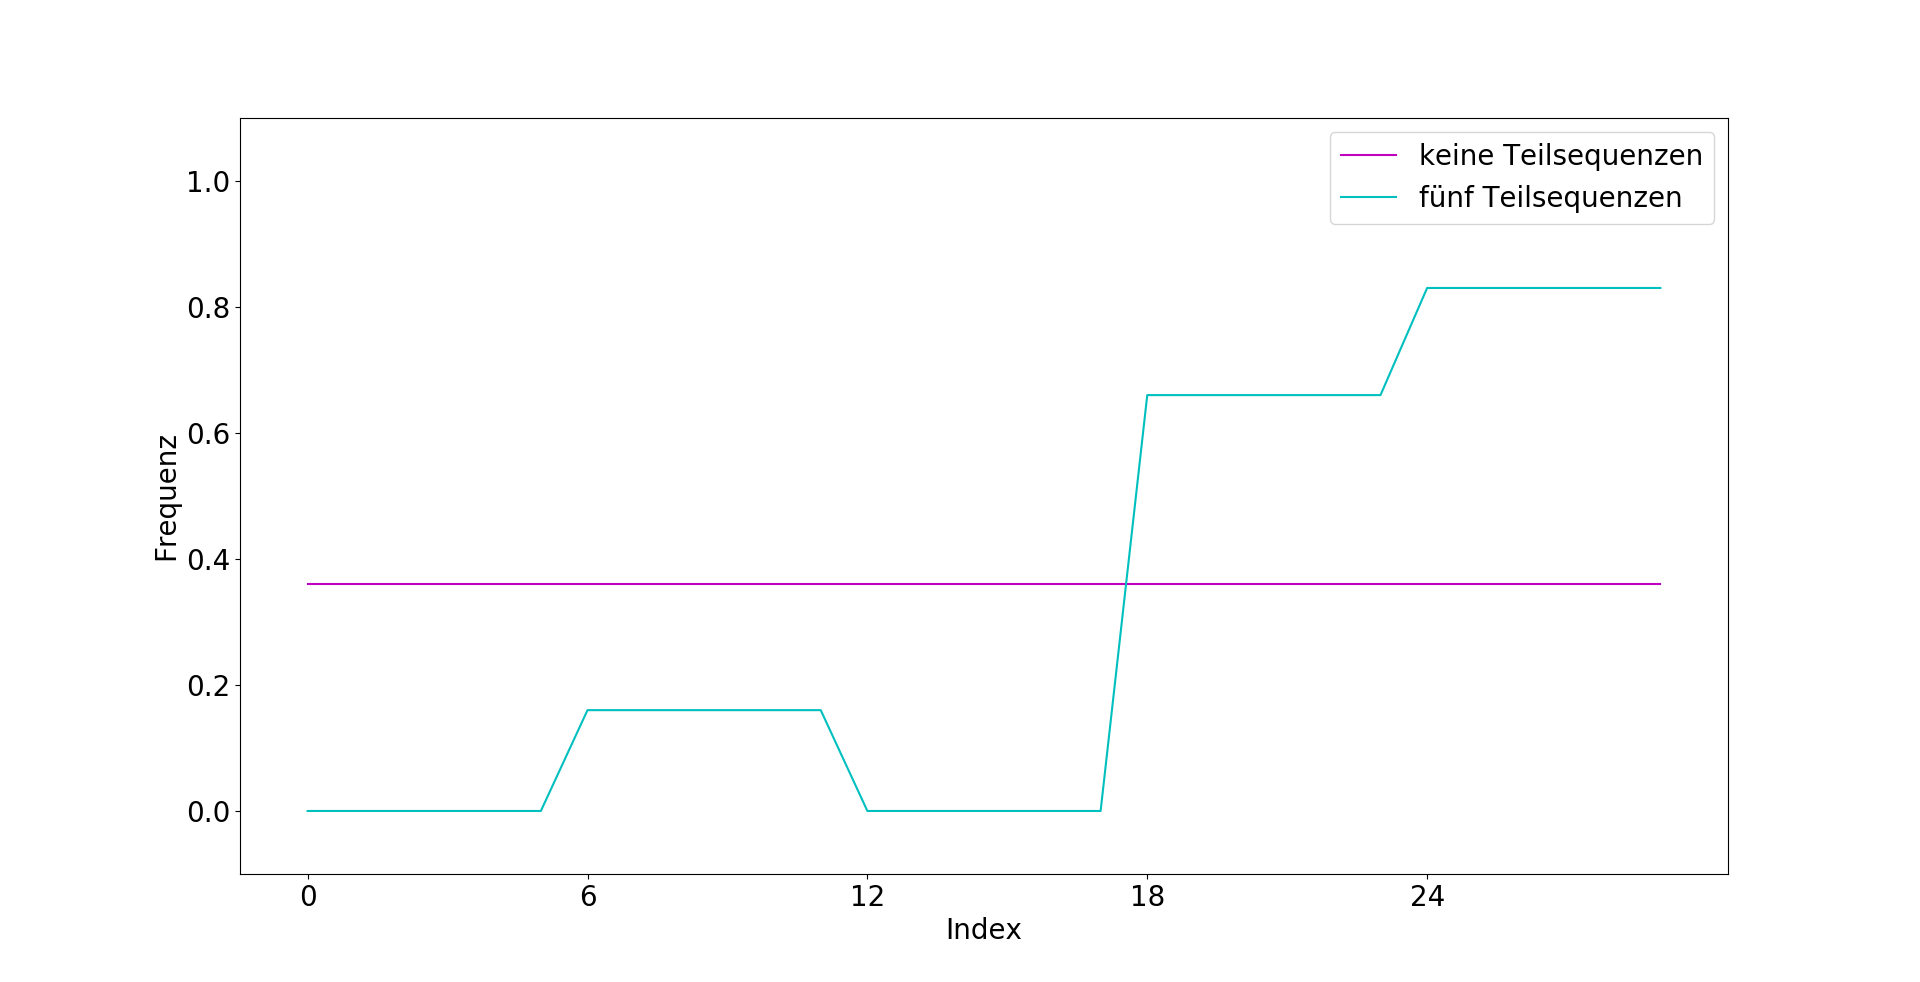
\includegraphics[scale=0.32]{images/sequences/subsequences-frequency}
	\caption{Frequenz ohne und mit fünf Teilsequenzen}
	\label{fig:properties-subsequences-frequency}
\end{figure}
\end{theorem}

\subsubsection{Wertebereich}

Der kleinste Wert für die Balance oder Frequenz ist 0 und der größte kleiner gleich 1. Eine Sequenz mit einer niedrigen, bzw. hohen Balance wird als unausgeglichen beschrieben, während ein Wert um die 0.5 als ausgeglichen gilt. Dieser Ausgleich bezieht sich letztlich auf die Verteilung der Nullen und Einsen. Eine detaillierte Auflistung der unterschiedlichen Wertebereiche findet sich in Tabelle~\ref{tab:properties-balance}. Da die Balance für zwei Zustände berechnet werden kann, wird der Einfachheit halber - wenn von Balance gesprochen wird - implizit die Balance von \textit{Fehlerzustand}, bzw. $B(1)$ angenommen. 

\begin{table}[H]
	\begin{center}
		\begin{tabular}{|c c|}
			\hline
			Balance & Beschreibung \\
			\hline\hline
			$0 \leq B < 0.4$ & unausgeglichen \\ 
			\hline
			$0.4 \leq B \leq 0.6$ & ausgeglichen \\
			\hline
			$0.6 < B \leq 1$ & unausgeglichen \\
			\hline
		\end{tabular}
		\caption{Balance}
		\label{tab:properties-balance}
	\end{center}
\end{table}

Da mit der Frequenz ein Maß für die Wertewechsel innerhalb einer Sequenz bildet, entspricht ein Wert gegen 0 einer sehr inaktiven Sequenz mit nur sehr wenigen bis keinen Wertewechseln. Ein Wert von 1 steht hingegen für eine hochfrequente Sequenz, in der sehr viel Wertewechsel stattfinden. Eine detaillierte Auflistung der unterschiedlichen Wertebereiche findet sich in Tabelle~\ref{tab:properties-frequency}. 

\begin{table}[H]
	\begin{center}
		\begin{tabular}{|c c|} 
			\hline
			Frequenz & Beschreibung \\
			\hline\hline
			$0 \leq F \leq 0.25$ & niederfrequent \\ 
			\hline
			$0.25 < F < 0.75$ & mittelfrequent \\
			\hline
			$0.75 \leq F < 1$ & hochfrequent \\
			\hline
		\end{tabular}
		\caption{Frequenz}
		\label{tab:properties-frequency}
	\end{center}
\end{table}

Mit der Balance und Frequenz sind nun zwei Eigenschaften definiert, mit denen sich grundsätzliche Aussagen über Sequenzen treffen lassen. Aus betriebswirtschaftlicher Sicht ist es erstrebenswert, die Balance von \textit{Fehlerzustand} möglichst niedrig zu halten. Eine Balance von 0 wäre der Idealzustand, da somit kein Fehlerzustand in der Sequenz vorhanden ist. 

Wenn man die Frequenz einer Sequenz betrachtet, lässt sich grundsätzlich sagen, dass eine niederfrequente Sequenz ein wünschenswerter Zustand ist, denn wenige Wertewechsel sprechen für eine gewisse Kontinuität und Stabilität. Allerdings sollte man die Frequenz zusammen mit der Balance und nicht alleine betrachten. Denn eine niedrige Frequenz im Zusammenspiel mit einer hohen Balance würde bedeuten, dass sich eine Maschine konstant im Fehlerzustand befindet.

\section{Korrelation}
\label{chp:correlation-sequences}
Bisher wurden Sequenzen nur für sich alleine betrachtet und nicht im Zusammenhang mit Anderen. Dabei scheint dies sogar notwendig, wenn man sich vergegenwärtigt, dass Fertigungslinien oft aus mehreren unterschiedlichen Produktionsmaschinen bestehen. Diese bilden untereinander oft Abhängigkeiten, weshalb das Auftreten zeitlicher Korrelation erwartbar ist. Eine solche zeitliche Verschiebung ist in Abbildung \ref{fig:correlation-sequences-corr} dargestellt. Hier lässt sich das Muster von Sequenz 1 in Sequenz 2 mit einer Verschiebung von 3 beobachten.  

\begin{figure}[H]
	\centering
	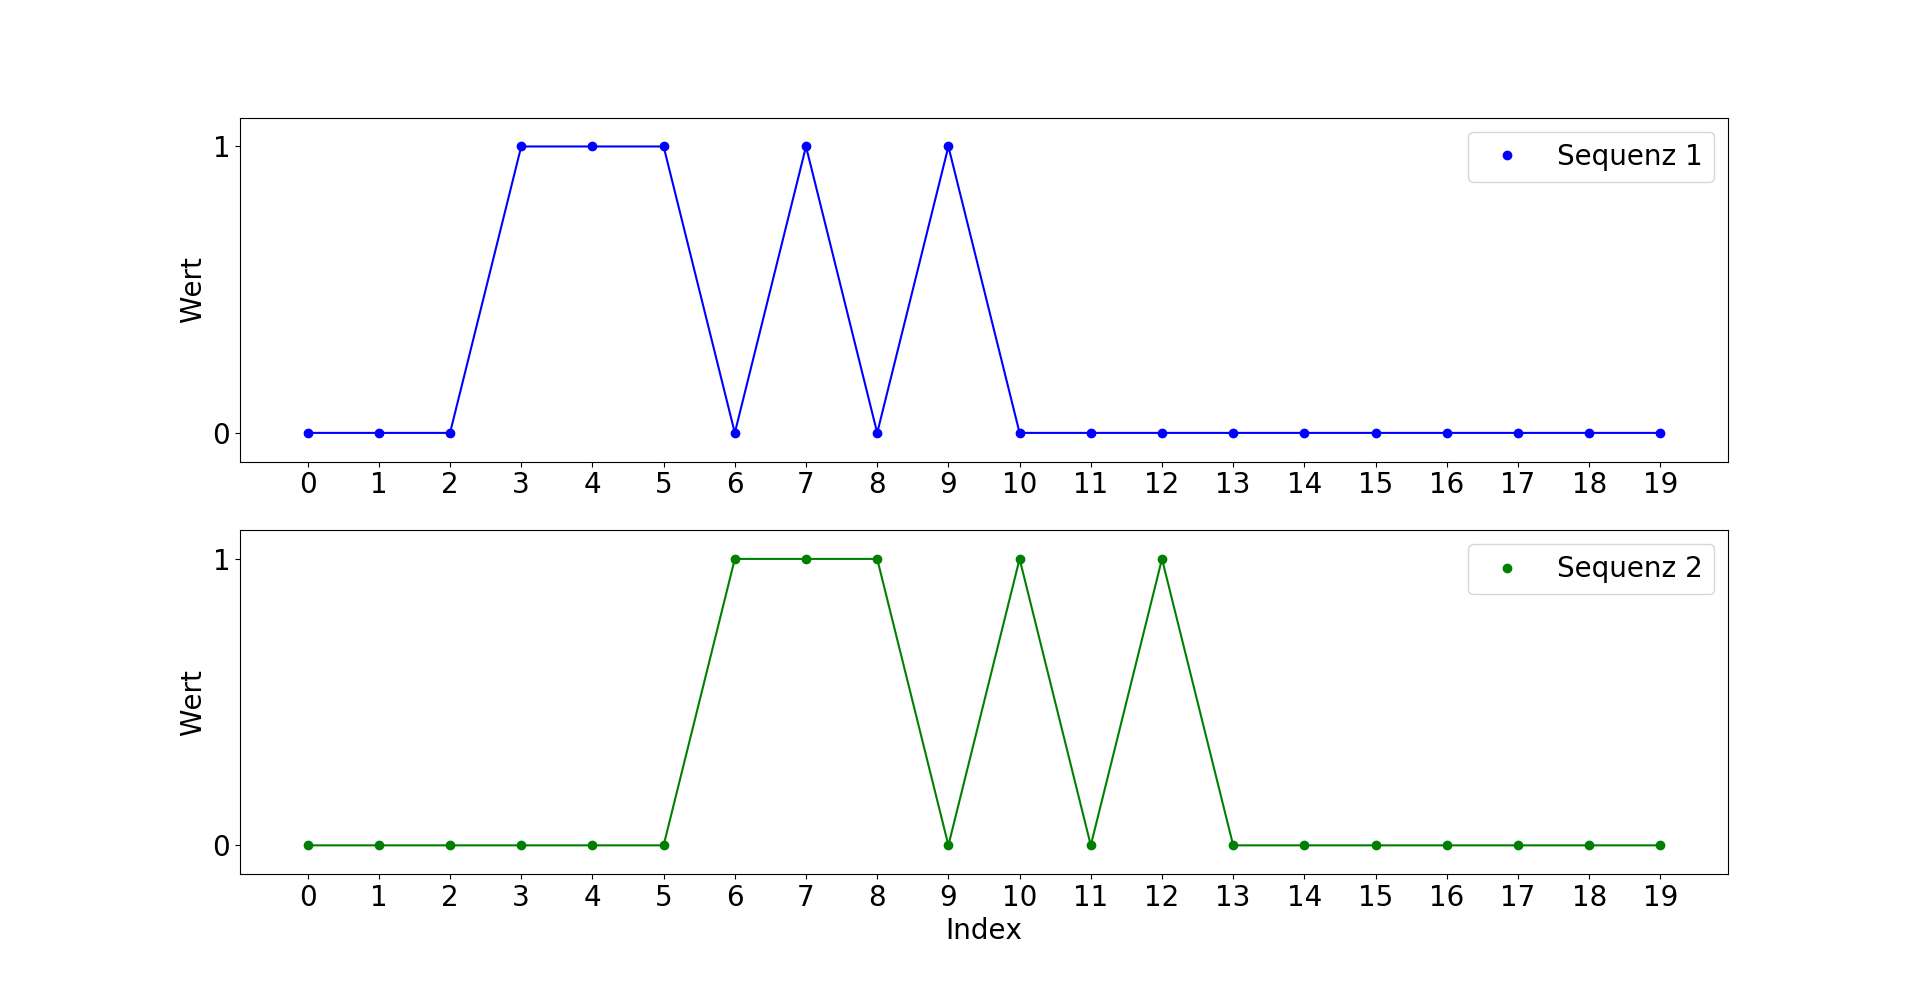
\includegraphics[scale=0.32]{images/sequences/correlation}
	\caption{Zeitliche Korrelation zwischen zwei Sequenzen}
	\label{fig:correlation-sequences-corr}
\end{figure}

Mit Hilfe der Korrelation als Maß für den Zusammenhang zwischen Sequenzen, wird eine solche Betrachtung möglich. In der Signalanalyse wird dafür die Kreuzkorrelationsfunktion verwendet. Auch wenn eine zeitliche Korrelation zwischen Sequenzen so nachgewiesen werden kann, ist dies noch kein Nachweis für einen kausalen Zusammenhang. Die Implementierung dieser Funktion sowie deren beispielhafte Verwendung findet sich in Kapitel \ref{chp:crosscorrelation:implementation}.

\section{Klassifizierung}
\label{chp:classification-sequences}
Wenn man Sequenzen graphisch darstellt ergeben sich unterschiedliche Muster. Um die Klassifikation von Sequenzen zu erleichtern, wurden in Kapitel \ref{chp:properties-sequences} die Wertebereiche für Balance und Frequenz definiert. Im Folgenden werden markante Muster, welche in Teilsequenzen auftreten können, beschrieben.

Das erste Muster nennt sich \textit{Ausreißer} und ist in Abbildung \ref{fig:classification-sequences-outlier} dargestellt. Eine solche Teilsequenz befindet sich fast ausschließlich in einem Zustand. Änderungen treten fast gar nicht und wenn doch nur kurz auf. Bei Produktionsprozessen kann man dieses Muster bei einer Maschine, welche im Regelbetrieb arbeitet und kurz einen Fehler wirft, beobachten. Wichtig dabei ist, dass schnell wieder ein Sprung in den Ausgangszustand stattfindet. Die Balance einer solchen Sequenz ist unausgeglichen und die Frequenz sehr niedrig.

\begin{figure}[H]
	\centering
	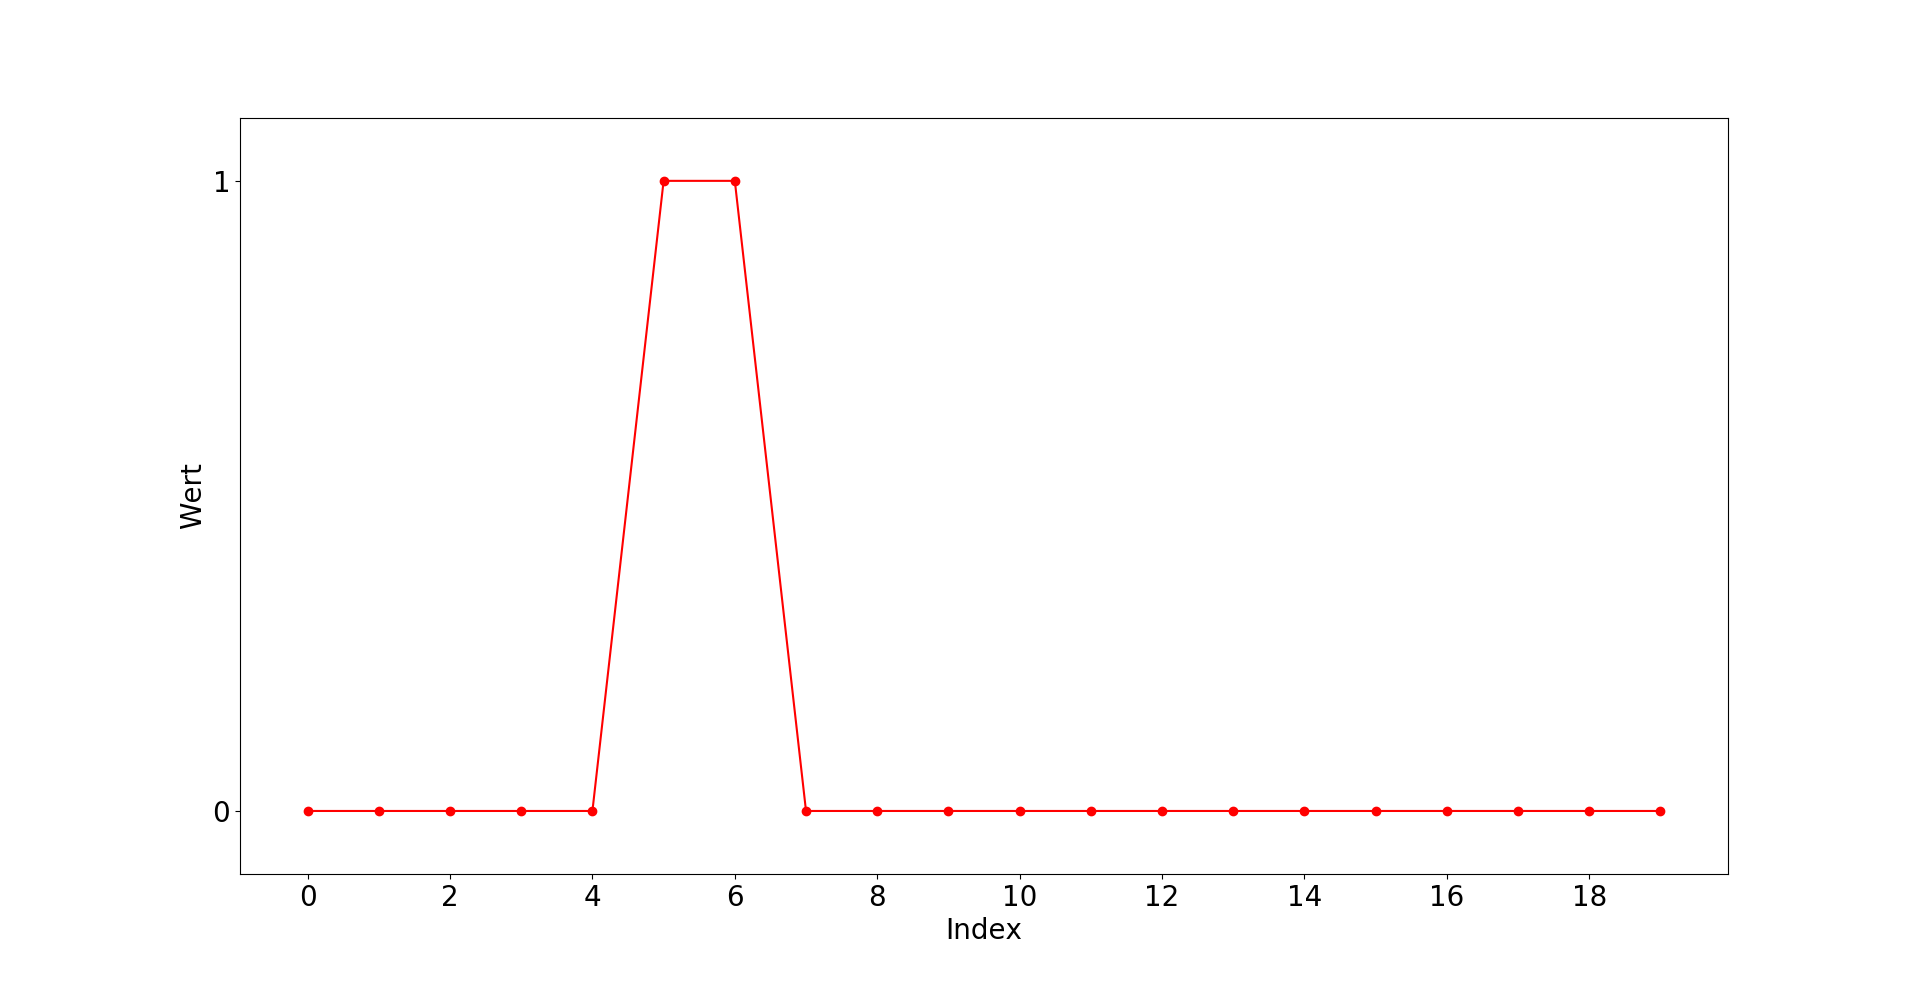
\includegraphics[scale=0.32]{images/sequences/outlier}
	\caption{Sequenz mit einem Ausreißer}
	\label{fig:classification-sequences-outlier}
\end{figure}

Ein weiteres Grundmuster ist in Abbildung \ref{fig:classification-sequences-tremor} dargestellt. Dieses zeigt einen regelmäßigen Wechsel zwischen den zwei möglichen Zuständen und wird als \textit{Zittern} bezeichnet. Dieses Verhalten ist eher untypisch für Produktionsmaschinen und dürfte nicht oft in der Realität beobachtet werden. Hier wäre ein Rückschluss auf eine defekte Sensorik naheliegend. Solche Sequenzen haben eine Balance von ca. 0.5 sowie eine hohe Frequenz .

Bei dem dritten Muster befindet sich eine Sequenz zuerst in einem Zustand und verharrt nach einem Wertewechsel im Anderen. Abbildung \ref{fig:classification-sequences-change} zeigt dieses Muster. In der Praxis kann so ein Muster auftreten, wenn eine Maschine im Regelbetrieb arbeitet und auf Grundlage eines Fehlers längere Zeit ausfällt. Durch diesen \textit{Wechsel} ergibt sich zudem der Name dieses Musters. Die Balance ist ausgeglichen und die Frequenz sehr niedrig.

\begin{figure}[H]
	\centering
	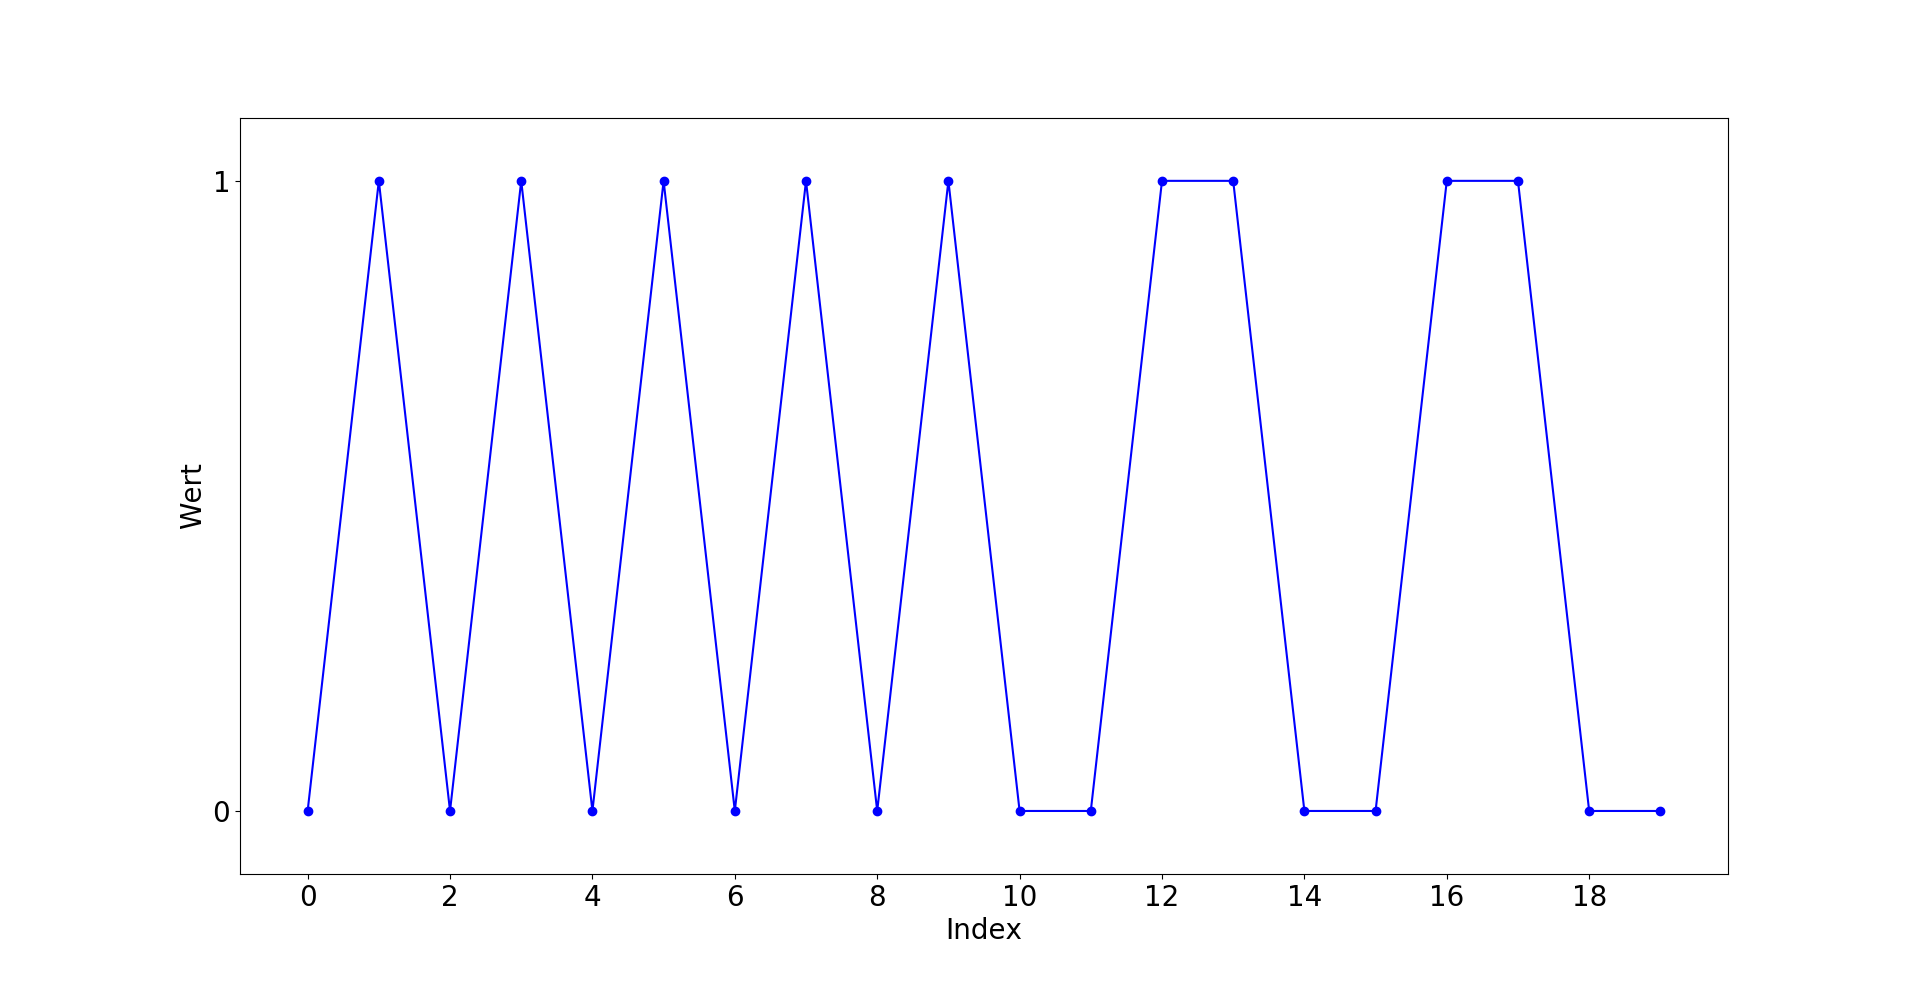
\includegraphics[scale=0.32]{images/sequences/tremor}
	\caption{Sequenz mit einem Zittern}
	\label{fig:classification-sequences-tremor}
\end{figure}

\begin{figure}[H]
	\centering
	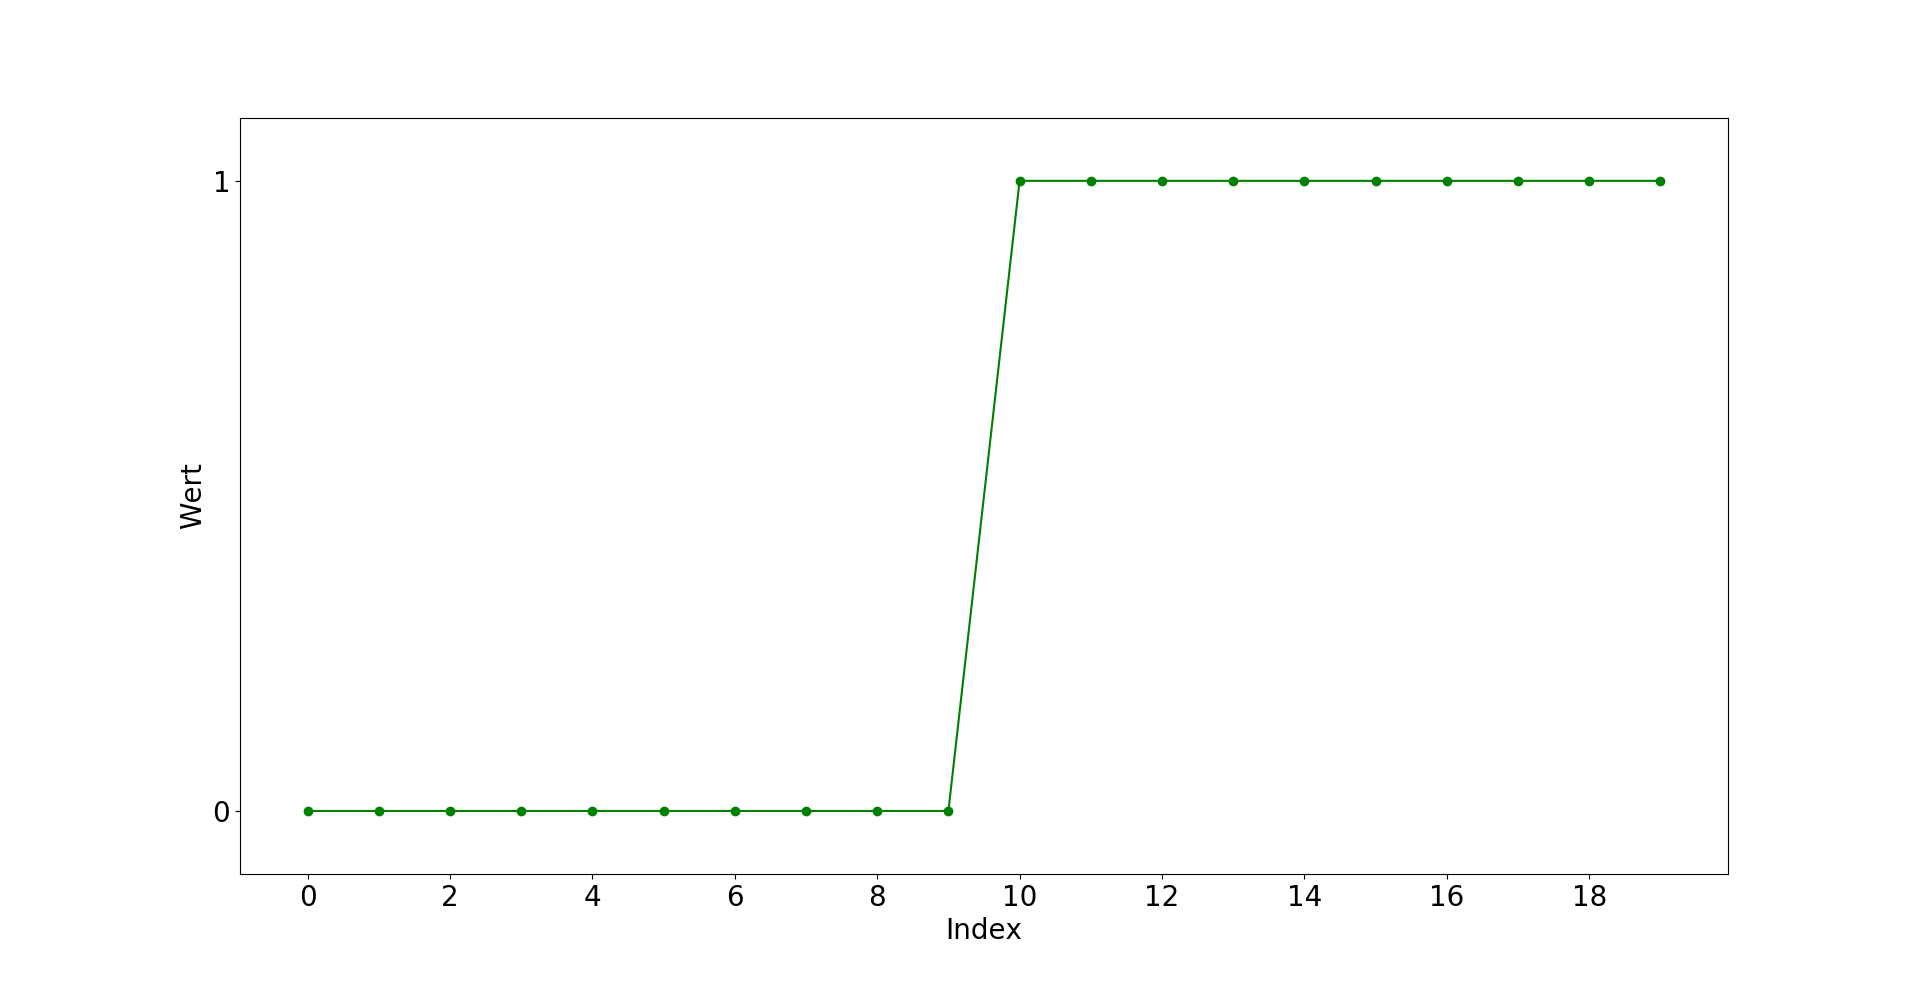
\includegraphics[scale=0.32]{images/sequences/change}
	\caption{Sequenz mit einem Wechsel}
	\label{fig:classification-sequences-change}
\end{figure}

Die bereits erwähnte Kreuzkorrelation findet auch Anwendung bei der Mustersuche in Sequenzen. Die Implementierung dieser Funktion und ihre Verwendung sind in Kapitel \ref{chp:crosscorrelation:patternsearch} dargestellt.